\documentclass{tufte-handout}
\usepackage{lmodern}
\usepackage{amssymb,amsmath}
\usepackage[T1]{fontenc}
\usepackage[utf8]{inputenc}
\usepackage{amsfonts}
\usepackage{tikz}
\usepackage{environ}
\usetikzlibrary{arrows, matrix, shapes, decorations, positioning}


\NewEnviron{definition}[1]{%
\vspace*{0.7cm}
\centering
\begin{tikzpicture}
\node [inner sep=10pt, inner ysep=15pt,fill=BrickRed!5] (box){%
\begin{minipage}{0.8\textwidth}
  \noindent\BODY
\end{minipage}
};

\node[right=0.5cm of box.north west, font=\sffamily, fill=BrickRed, text=white,
 rounded corners] (m) {#1};
\draw[BrickRed, thick] (box.north west) -- (m.west);
\draw[BrickRed, thick] (m.east) -- (box.north east);
\draw[BrickRed, thick] (box.south west) -- (box.south east);
\end{tikzpicture}
\vspace*{0.7cm}
}

\tikzstyle{simpletable}=[matrix of nodes,inner sep=0pt, nodes in empty cells,
nodes={draw=gray, ultra thin, minimum size=1cm,anchor=center,align=center},
row 1/.style={nodes={anchor=center, font=\bf}},
column 1/.style={nodes={align=center, anchor=center,font=\bf}},
row 1 column 1/.style={nodes={draw=white, ultra thin, anchor=center}}]
\tikzstyle{marked}=[fill=BrickRed!10]

% section format
\titleformat{\subsection}%
  {\sffamily\Large\itshape\color{BrickRed}}% format applied to label+text
  {}% label
  {}% horizontal separation between label and title body
  {}% before the title body
  []% after the title body

  % subsection format
\titleformat{\section}%
  {\sffamily\huge\color{BrickRed}}% format applied to label+text
  {}% label
  {}% horizontal separation between label and title body
  {}% before the title body
  [\vspace*{5mm}]% after the title body

\newcommand{\sectionbreak}{\clearpage}

\title{}
\author{Pablo Baeyens}
\date{}

\begin{document}

\section{Pure Strategies}

\subsection{Self-interested agents}

A \emph{self-interested} agent is an agent that has preferences over
certain states of the world. This is formalized by utility functions\footnote{
The usefulness of utility functions is shown in the
\textbf{Von Neumann–Morgenstern utility theorem} which derives its existence
from some basic axioms.}:

\begin{definition}{Utility function}
A \textbf{utility function} is a function $u: S \to \mathbb{R}$
that describes the likings of an agent.

Given a state $s \in S$, $u(s)$ is its \textbf{utility}.
\end{definition}

An agent is \textbf{rational} if they maximize expected utility.

\vspace*{1cm}

\subsection{Games}

The basic elements for a game are players, actions and their payoffs:

\begin{definition}{Finite $n$-person normal form game}
  A \textbf{finite $n$-person normal form game} is a
  $3$-tuple $\langle N, A, u\rangle$ where:
  \begin{itemize}
  \item $N = \{1,\dots, n\}$ are the \textbf{players}
  \item $A = A_1 \times \dots \times A_n$ are the \textbf{actions}.

        $a = (a_i)_{1..n} \in A$ is an \textbf{action profile}.
  \item $u_i: A \to \mathbb{R}$ the \textbf{utility function} of player $i$.
  \end{itemize}
\end{definition}

\begin{marginfigure}
\smallcaps{Prisoner's dilemma}

\begin{center}
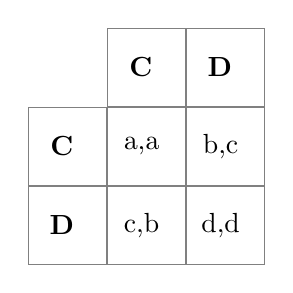
\begin{tikzpicture}
\node [simpletable] {
& C & D \\
C & a,a & b,c \\
D & c,b & d,d \\
};
\end{tikzpicture}
\end{center}
\vspace*{2mm}

A prisoner's dilemma is a $2$-player game where $c > a > d > b$.

The possible actions are to \textbf{C}ooperate or to \textbf{D}efect.
The classical example involves two incommunicated prisoners which
committed a joint crime. They are told that:

\begin{itemize}
  \item If both cooperate (remain silent) they both get 1 year.
  \item If one defects he gets 0 years and the other gets 4 years.
  \item If both defect they both get 3 years.
\end{itemize}
\end{marginfigure}


Games can be of different types:

\begin{itemize}
\item A $2$-player game is of \textbf{pure competition} if
\[ \forall a \in A: \; u_1(a) + u_2(a) = c\]
If $c = 0$ it's a \textbf{zero sum game}.
\item A game is of \textbf{pure coordination} if
\[\forall a \in A: \forall i,j: \; u_i(a) = u_j(a)\]
\end{itemize}

\pagebreak

\subsection{Nash Equilibrium}

A Nash Equilibrium is an strategy profile in which:

\begin{itemize}
\item  Each player's strategy maximizes their utility given the others' actions.
\item  Nobody has an incentive to deviate from their action.
\end{itemize}

\begin{marginfigure}
\smallcaps{Example: Coordination game}

\begin{center}
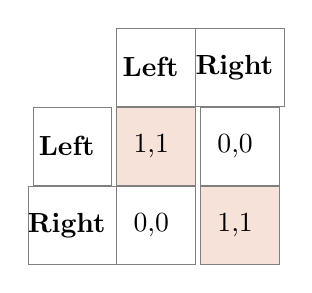
\begin{tikzpicture}
\node [simpletable,
row 2 column 2/.style={nodes={marked, anchor=center}},
row 3 column 3/.style={nodes={marked, anchor=center}}] {
& Left & Right \\
Left & 1,1 & 0,0 \\
Right & 0,0 & 1,1 \\
};
\end{tikzpicture}
\end{center}
\vspace*{2mm}

The classical $2$-player coordination game consists in
two players deciding on which side of the street they'll walk.
If they walk by the same side they won't collide with each other,
otherwise they will.

\vspace*{2mm}

This game has two pure Nash equilibria, shown in grey.
\end{marginfigure}


Let $a_{-i} = \langle a_1, \dots, a_{i-1}, a_{i+1}, \dots, a_n \rangle$.
Then:

\begin{definition}{Best response}
$a_i^* $ is a \textbf{best response} of $a_{-i}$ if:

$$\forall a_i \in A_i: u_i(a_i^*, a_{-i}) \geq u_i(a_i, a_{-i})$$
\end{definition}

Thus:

\begin{definition}{Nash equilibrium}
$a = \langle a_1, \dots, a_n \rangle$ is a (pure strategy)
\textbf{Nash equilibrium} if all $a_i$ are best responses of $a_{-i}$.
\end{definition}

\subsection{Dominant strategies}

A strategy is a possible course of action\footnote{This will be defined with
more detail later on in this document, but by now it can be considered as
choosing a certain action. This is also called a \textbf{pure strategy}}.
We will denote a strategy of player $i$ by $s_i$ or $s'_i$ and
the set of possible strategies of the other players by $S_{-i}$ Then:

\begin{definition}{Dominance}
$s_i$ \textbf{strictly dominates} $s'_i$ if
  \[\forall s_{-i} \in S_{-i}, u_i(s_i, s_{-i}) > u_i(s'_i, s_{-i})\]

$s_i$ \textbf{very weakly dominates} $s'_i$ if
  \[\forall s_{-i} \in S_{-i}, u_i(s_i, s_{-i}) \geq u_i(s'_i, s_{-i})\]
\end{definition}

\begin{marginfigure}
\smallcaps{Example: Dominance}

\vspace*{5mm}

In a prisoner's dilemma \textbf{D}efect is dominant.

\begin{center}
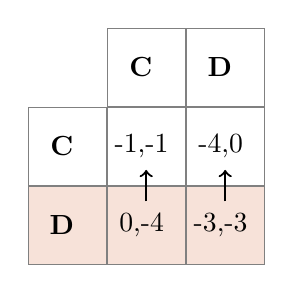
\begin{tikzpicture}
\node (m) [simpletable, row 3/.style={nodes={anchor=center, marked}}] {
& C & D \\
C & -1,-1 & -4,0 \\
D & 0,-4 & -3,-3 \\
};
\node[below = 2mm of m-2-2] (a) {};
\node[above = 2mm of m-3-2] (b) {};
\draw[->, thick] (a) -- (b);
\node[below = 2mm of m-2-3] (c) {};
\node[above = 2mm of m-3-3] (d) {};
\draw[->, thick] (c) -- (d);
\end{tikzpicture}
\end{center}
\end{marginfigure}

If one strategy dominates all others, it is \textbf{dominant}.

\subsection{Pareto optimality}

Pareto dominance is a way to define an order relation between
action profiles in order to find which one is best from a global
perspective\footnote{Utilities of different players can't be added
thus we shouldn't use total or average utility as global measures.}.

\begin{marginfigure}
\smallcaps{Example: Battle of the Sexes}

\begin{center}
\begin{tikzpicture}
\node [simpletable,
row 2 column 2/.style={nodes={marked, anchor=center}},
row 3 column 3/.style={nodes={marked, anchor=center}}] {
& B & R \\
B & 2,1 & 0,0 \\
R & 0,0 & 1,2 \\
};

\node[above = 3mm of m-2-2.south] (a) {};
\node[below = 3mm of m-3-2.north] (b) {};
\draw[->, thick] (a) -- (b);
\node[above = 3mm of m-2-3.south] (c) {};
\node[below = 3mm of m-3-3.north] (d) {};
\draw[->, thick] (d) -- (c);
\node[left = 3mm of m-2-2.east] (e) {};
\node[right = 2mm of m-2-3.west] (f) {};
\draw[->, thick] (e) -- (f);
\node[left = 3mm of m-3-2.east] (g) {};
\node[right = 2mm of m-3-3.west] (h) {};
\draw[->, thick] (h) -- (g);
\end{tikzpicture}
\end{center}
\vspace*{2mm}

There are two Pareto-optimal outcomes in this game: the ones in which
both go watch the same film. These outcomes Pareto-dominate the others.

\end{marginfigure}

\begin{definition}{Pareto Optimality}
  An action profile $a$ \textbf{Pareto-dominates} $a'$ if
  \[ \forall a_i \in a, a'_i \in a', u_i(a_i) \geq u_i(a'_i)
  \; \wedge \; \exists j: \; u_j(a_j) > u_j(a'_j)\]
  That is: $a$ is better for every player and strictly
  better for at least one player.

  An action profile is \textbf{Pareto-optimal} if it isn't
  Pareto-dominated by any other outcome.
\end{definition}

A game can have more than one Pareto-optimal outcome and every game
has at least one Pareto-optimal outcome.

\section{Mixed Strategies}

In some games the best option is to randomize your strategy, in order to
become unpredictable or to deal with uncertainty. In the past section we
talked about pure strategies. Let us now generalize the concept:

\begin{definition}{Strategy}\label{strategy}
  A \textbf{strategy} $s_i$ for player $i$ is a probability distribution
  over the actions $A_i$.

  The \textbf{support} $\operatorname{Sup}(s_i)$ of a strategy
  is the set of actions with positive probability.
  If $\operatorname{Sup}(s_i)$ is $1$ $s_i$ is pure;
  otherwise it's mixed.
\end{definition}

We can calculate the \textbf{expected utility} of a strategy:

\begin{itemize}
  \item $u_i(s) = \sum_{a \in A} u_i(a)P(a|s)$
  \item $P(a|s) = \prod_{j \in N} s_j(a_j)$
\end{itemize}

We can now generalize the notions of best response and Nash equilibria by
talking about strategies
\footnote{It suffices to replace all mentions of actions by strategies
in the previously given definition.}:

\begin{definition}{Nash equilibrium}
$s = \langle s_1, \dots, s_n \rangle$ is a
\textbf{Nash equilibrium} if all $s_i$ are best responses of $s_{-i}$.
\end{definition}

This new definition allows us to state the following theorem:


\end{document}
